\documentclass[12pt,a4paper]{article}

% Packages for improved formatting
\usepackage[utf8]{inputenc}
\usepackage[T1]{fontenc}
\usepackage{lmodern}
\usepackage{microtype}
\usepackage[margin=1in]{geometry}
\usepackage{setspace}
\usepackage{sectsty}
\usepackage{titlesec}
\usepackage{alphabeta}
\usepackage{xcolor}
\usepackage{tikz}
\usepackage{amssymb}
\usepackage{lipsum}

% Customize section and subsection formatting
\titleformat{\section}{\normalfont\fontsize{14}{16}\bfseries}{\thesection}{1em}{}
\titleformat{\subsection}{\normalfont\fontsize{12}{14}\bfseries}{\thesubsection}{1em}{}
\titleformat{\subsubsection}[runin]{\normalfont\fontsize{12}{14}\bfseries}{\thesubsubsection}{1em}{}[:]

% Set line spacing
\onehalfspacing

% Add image
\graphicspath{ {./run.jpg}}
\graphicspath{ {./exampleRun.jpg}}

\begin{document}

\begin{titlepage}
    \begin{center}
        \vspace*{1cm}
        
        \Huge
        \textbf{Ψηφιακές Επικοινωνίες - Εργασία Αλγόριθμος CRC}
        
        \vspace{1.5cm}
        
        \Large
        Δεληγιαννάκης Χαράλαμπος

	\Large
	4383
        
        \vfill
        
        
        
        \Large
        Ιούνιος 2024
        
    \end{center}
\end{titlepage}

\section*{Εισαγωγή}
Στην εργασία παρουσιάζεται η υλοποίηση του αλγορίθμου CRC (Cyclic Redundancy Check), ο οποίος αποτελεί έναν από τους πιο γνωστούς κώδικες ανίχνευσης σφαλμάτων στη μετάδοση δεδομένων.

\section{Πρώτο ζητούμενο}   % Adds first section
Ο αλγόριθμος γράφτηκε σε γλώσσα Python και τα αρχεία έχουν ονόματα \textit{"main.py"} και \textit{"package.py"}.\\\\
Η βασική κλάση του αρχείου είναι η κλάση \textbf{Package} όπου υλοποιείται στο \textit{"package.py"} περιλαμβάνει όλες τις απαραίτητες πληροφορίες του πακέτου με τα δεδομένα (όπως τις μεταβλητές D, F, T, P της εκφώνησης) καθώς και όλες τις απαραίτητες λειτουργίες του αλγορίθμου CRC (modulo-2 binary division). Ουσιαστικά, η υλοποίηση του αλγορίθμου βρίσκεται μέσα σε αυτήν την κλάση. Ας αναλύσουμε κάθε μέθοδό της αναλυτικότερα:
\begin{itemize}
  \item Κατασκευαστής κλάσης:\\Δέχεται ως παραμέτρους τις μεταβλητές $D$ (η προς μετάδοση ακολουθία δεδομένων των $k$ bits) και $P$ (ο προκαθορισμένος αριθμός των $n-k+1$ bits με τον οποίο θα πρέπει να είναι διαιρέσιμη η ακολουθία των n bits που πρόκειται να μεταδοθεί).
  \item Μέθοδος send():\\Το πακέτο υποτίθεται ότι στάλθηκε και στη συγκεκριμένη μέθοδο καλούνται οι 4 παρακάτω υπομέθοδοι με τη σειρά για να υλοποιήσουν τον αλγόριθμο CRC.
  \begin{enumerate}
    \item Μέθοδος calculateF():\\Υπολογίζει την ακολουθία FCS ($F$) των $n-k$ bits, εκτελώντας την modulo-2 διαίρεση του $2^{n-k}D$ με το $P$ και χρησιμοποιώντας το υπόλοιπο αυτής.
    \item Μέθοδος calculateT():\\Υπολογίζει την ακολουθία $T$ των n bits που πρόκειται να μεταδοθεί, εκτελώντας την πράξη $2^{n-k}D+F$.
    \item Μέθοδος errors():\\Προσομοιώνει την δημιουργία σφαλμάτων κατά τη μετάδοση. Στον συγκεκριμένο κώδικα το bit error rate είναι $10^{-3}$.
    \item Μέθοδος calculateRes():\\Υπολογίζει το υπόλοιπο της modulo-2 διαίρεσης του $T$ με το $P$, το οποίο δείχνει αν υπήρχε σφάλμα κατά τη μετάδοση. (Αν υπήρχε, είναι διάφορο του μηδενός)
  \end{enumerate}
  \item Μέθοδος xor():\\Υπολογίζει το αποτέλεσμα της γνωστής πράξης XOR μεταξύ δύο δυαδικών αριθμών που είναι σε μορφή String.
  \item Μέθοδος binary\_division():\\Υπολογίζει το υπόλοιπο της modulo-2 διαίρεσης δύο δωαδικών αριθμών.
\end{itemize}
Στο αρχείο \textit{"main.py"}, για το πρώτο ζητούμενο δημιουργείται τυχαία αριθμός $k$ μεταξύ 10 και 30 όπου αντιπροσωπεύει το μέγεθος της πληροφορίας σε bits. Έπειτα, ζητείται από τον χρήστη να εισάγει τον σταθερό αριθμό $P$ και τέλος δημιουργούνται 10 τυχαία μηνύματα (μεγέθους $k$ bits το καθένα) τα οποία στέλνονται και ελέγχονται από τον αλγόριθμο. Ένα παράδειγμα εκτέλεσης είναι το εξής:
\begin{figure}[h]
    \centering
    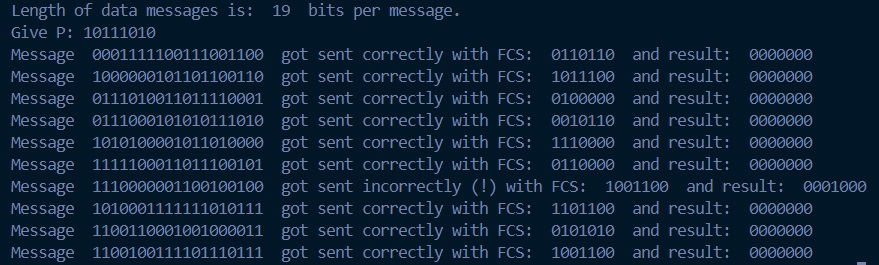
\includegraphics[width=0.8\textwidth]{exampleRun}
    \caption{Έξοδος τυχαίας εκτέλεσης του προγράμματος για το πρώτο ζητούμενο}
    \label{fig:example}
\end{figure}

\section{Δεύτερο ζητούμενο}   % Adds second section
Η εκτέλεση για τα δεδομένα του δεύτερου ζητουμένου υλοποιείται στη συνάρτηση\\ $randomPackages()$ του αρχείου \textit{"main.py"}. Σε αυτήν, δημιουργούνται αντικείμενα της κλάσης Package, όπου σε κάθε πακέτο μεταδίδεται μια ακολουθία με συγκεκριμένο μέγεθος. Στη συνέχεια, για κάθε πακέτο καλείται η μέθοδος send(), και τυπώνονται τα κατάλληλα βοηθητικά μηνύματα του δεύτερου ζητούμενου. Τονίζεται πως για να τρέξει το δεύτερο ζητούμενο, πρέπει η γραμμή 36 στο main αρχείο να μην είναι commented, δηλαδή να γίνει η εξής αλλαγή: \textit{\#randomPackages() -> randomPackages()}\\\\
Ο παραπάνω αλγόριθμος έτρεξε για δεδομένα με μήκος πληροφορίας $k=20$ bits, $P=110101$ και bit error rate $BER=10^{-3}$. Τα αποτελέσματα που παρήχθηκαν είναι τα εξής:
\begin{itemize}
  \item Αριθμός πακέτων: 1000 πακέτα
  \item Το ποσοστό των μηνυμάτων που φθάνουν με σφάλμα (στο block δεδομένων ή στο CRC) στον αποδέκτη: 2.6\%
  \item Το ποσοστό των μηνυμάτων που ανιχνεύονται ως εσφαλμένα από το CRC: 2.5\%
  \item Tο ποσοστό των μηνυμάτων που φθάνουν με σφάλμα στο αποδέκτη και δεν ανιχνεύονται από το CRC: 0.1\%
\end{itemize}
\begin{figure}[h]
    \centering
    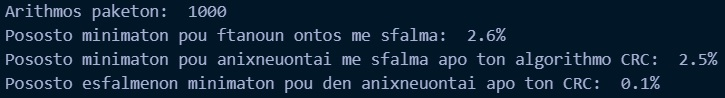
\includegraphics[width=0.8\textwidth]{run}
    \caption{Έξοδος τυχαίας εκτέλεσης του προγράμματος για το δεύτερο ζητούμενο}
    \label{fig:run}
\end{figure}
Γενικά, ο αλγόριθμος CRC δεν ανιχνεύει όλα τα σφάλματα. Αυτό φαίνεται και στην παραπάνω εκτέλεση. Όμως, επειδή η παραγωγή των πληροφοριών είναι τυχαία, υπάρχει προφανώς μεγάλη περίπτωση να υπάρχουν εκτελέσεις όπου ο αλγόριθμος ανιχνεύει όλα τα σφάλματα. Πράγματι, αν ο αλγόριθμος τρέξει για 1000 πακέτα όπως και πάνω, σχεδόν όλες τις φορές ο αλγόριθμος θα ανιχνεύσει όλα τα σφάλματα. Μεγαλύτερος αριθμός πακέτων δίνει μεγαλύτερες πιθανότητες να μην ανιχνεύσει ο αλγόριθμος κάποιο υπάρχον σφάλμα στη μετάδοση ενός πακέτου.
\end{document}
